\documentclass{sigchi}

% Use this command to override the default ACM copyright statement (e.g. for preprints). 
% Consult the conference website for the camera-ready copyright statement.
\toappear{}



% Arabic page numbers for submission. 
% Remove this line to eliminate page numbers for the camera ready copy
\pagenumbering{arabic}


% Load basic packages
\usepackage{balance}  % to better equalize the last page
\usepackage{graphics} % for EPS, load graphicx instead
\usepackage{times}    % comment if you want LaTeX's default font
\usepackage{url}      % llt: nicely formatted URLs

% llt: Define a global style for URLs, rather that the default one
\makeatletter
\def\url@leostyle{%
  \@ifundefined{selectfont}{\def\UrlFont{\sf}}{\def\UrlFont{\small\bf\ttfamily}}}
\makeatother
\urlstyle{leo}


% To make various LaTeX processors do the right thing with page size.
\def\pprw{8.5in}
\def\pprh{11in}
\special{papersize=\pprw,\pprh}
\setlength{\paperwidth}{\pprw}
\setlength{\paperheight}{\pprh}
\setlength{\pdfpagewidth}{\pprw}
\setlength{\pdfpageheight}{\pprh}

% Make sure hyperref comes last of your loaded packages, 
% to give it a fighting chance of not being over-written, 
% since its job is to redefine many LaTeX commands.
\usepackage[pdftex]{hyperref}
\hypersetup{
pdftitle={SIGCHI Conference Proceedings Format},
pdfauthor={LaTeX},
pdfkeywords={SIGCHI, proceedings, archival format},
bookmarksnumbered,
pdfstartview={FitH},
colorlinks,
citecolor=black,
filecolor=black,
linkcolor=black,
urlcolor=black,
breaklinks=true,
}

% create a shortcut to typeset table headings
\newcommand\tabhead[1]{\small\textbf{#1}}


% End of preamble. Here it comes the document.
\begin{document}
\nocite{*}
\title{Campus Sherpa}

\numberofauthors{4}
\author{
  \alignauthor Christopher Ford\\
    \email{cjford@mit.edu}\\
  \alignauthor Ganesh Ajjanagadde\\
    \email{gajjanag@mit.edu}\\  
  \alignauthor Harihar Subramanyam\\
    \email{hsubrama@mit.edu}\\
   \alignauthor James Thomas\\
    \email{jjthomas@mit.edu}\\
}

\maketitle

\begin{abstract}
In this paper, we outline the motivation, development, and testing of Campus Sherpa, a mobile application for iOS 7 that allows users to make and take custom tours of the Massachusetts Institute of Technology (MIT) campus. The app was inspired by a generative study which showed that people were unhappy with the one-size-fits-all approach of traditional campus tours and desired a tourism experience which catered to the varying interests of tourists. Campus Sherpa was developed to allow users to create and takes tours of the MIT campus. It serves as a platform for students to make tours to remember their experience at MIT, and for visitors to take tours which cater to their interests at MIT. Our field evaluation, conducted after the development of our application, showed that Campus Sherpa was well suited to improve upon the tour taking experience at MIT. 
\end{abstract}

\keywords{
	Geolocations; campus; tours; location tracking; tourism; college; sharing
}
% Stubbed out these sections for now, don't know what to do with them

%\keywords{
%	Guides; instructions; author's kit; conference publications;
%	keywords should be separated by a semi-colon.
%	\textcolor{red}{Mandatory section to be included in your final version.}
%}
%
%\category{H.5.m.}{Information Interfaces and Presentation (e.g. HCI)}{Miscellaneous}
%
%See: \url{http://www.acm.org/about/class/1998/}
%for more information and the full list of ACM classifiers
%and descriptors. 
%\textcolor{red}{Mandatory section to be included in your
%final version. On the submission page only the classifiers'
%letter-number combination will need to be entered.}

\section{Introduction}

Every day, MIT receives a large number of visitors from different backgrounds. 

\begin{figure}[h]
\centering
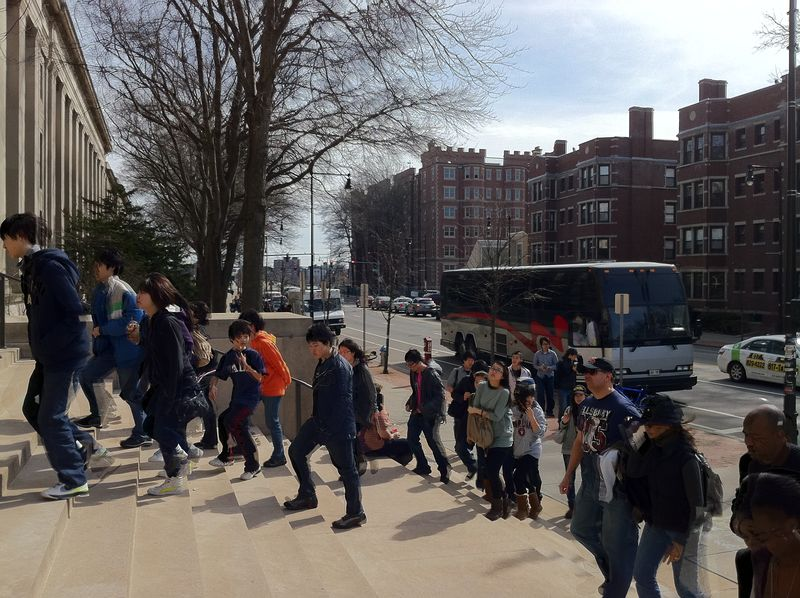
\includegraphics[width=1.0\linewidth]{./Tourists}
\caption{A large group of tourists on MIT's campus}
\label{fig:Tourists}
\end{figure}

The visitors include tourists exploring Boston/Cambridge, prospective undergrads, prospective grad students, middle/high schoolers attending Splash, researchers attending a conference, and professionals attending an event or career fair. Each visitor has different interests when visiting MIT. For instance, an incoming freshman may be focused on exploring the undergraduate residences while a prospective biology graduate student may be more interested in the biological research labs. However, many of these visitors take campus tours which take them to the main sights at MIT (e.g. the Student Center, gymnasium, auditorium, main hallway, and architecturally impressive computer science laboratory). However, this ``one-size-fits-all'' nature of the tour fails to take into account the interests of each visitor and show them all the sights that they would enjoy seeing. 

Campus Sherpa is a tourism app focused on MIT. Users can create tours, which are sequences of locations associated with media (e.g. pictures, audio narration). Users can take tours, which takes them on a guided trip to interesting sites on the MIT campus and shows them relevant media for each site.

Primary research questions include: ``How can we fix this with an easy to use mobile application?", ``Is a mobile application the right way to solve this problem?", and ``How can we take advantage of modern cell phone technologies to make use of our application as easy as possible?"

One goal of this application is to allow users to pursue a tour (likely after the main campus tour) which will help them make the most of their time at MIT. For instance, a prospective graduate student in Biology would follow a tour of the biology labs while a tourist interested in history would be taken to the most historically important sites at MIT. 

The second aspect of this application is to allow users to chronicle their tours and share them with others. As prospective students compare MIT to other schools or as tourists reminisce about their visit to MIT, the ability to record their tours (by associating locations with text, photos, videos, and links to related content) will aid them in remembering. For current students, this offers a way to record the precious memories they make at MIT and share them with others.

Since smartphones offer location awareness and mobility, they are the obvious platform choice for this application. By deploying this application for iOS, users can take out their smartphone when they arrive at MIT, select a tour based on their interests, and then begin exploring sites that will be most useful to them. Also, they can create a tour so that they can revisit their memories later on. 

Thus, the primary audience will be people who aim to tour MIT and record their experience there. The secondary audience will be current MIT students who would like to chronicle their lives at MIT. While some MIT tours will be pre-installed, the majority are intended to be user-created. 

Based on our own experiences and the results of our interviews, people have varied tastes and desired destinations when visiting MIT. We therefore aimed to make sure that their trip to MIT is as enjoyable and productive as possible. By creating an application to let users create, share, and follow custom tours of MIT, we hoped to make college tours custom fit to each person's taste, to make memories of MIT easy to record and share, and to make a platform for sharing tours.

\section{Related Work}

There exist a number of products and applications aimed at making tour taking more exciting and enjoyable. Interactive exhibits at museums and college campuses aim to improve upon the tour taking experience by allowing tour takers to interact with what they are touring. These interactive kiosks often serve many tourists at once, and fail to provide a custom tailored experience to each user. Often, these interactive stations can get bogged down with traffic, resulting in long wait times which only frustrates the tourist.

There exist a few mobile applications that try to enrich tourism as well. Applications in this domain fall into two main categories: applications that try to replace the tour taking experience all together, and applications that try to supplement existing tours. Applications in the first category include the Library of Congress Virtual Tour, Canadian Museum of Civilization, and the American Museum of Natural History mobile applications.

\begin{figure}[h]
\centering
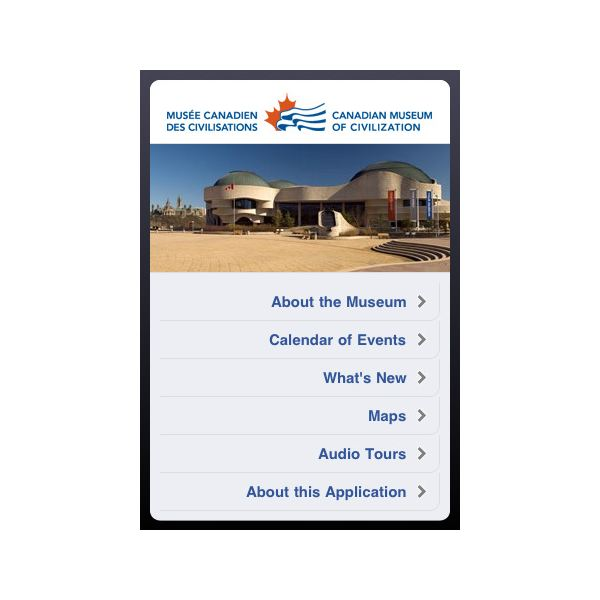
\includegraphics[width=1.0\linewidth]{./CanadianMuseumOfCivilization}
\caption{The main screen of the Canadian Museum of Civilization app. One drawback of this app is that it does not support user generated tours.}
\label{fig:CanadianMuseumOfCivilization}
\end{figure}

Although these virtual tours allow more users to ``explore'' a tourist destination, they fail to replicate the experience of touring in person. A 3.5 inches to 5 inches screen is not a good way to replicate a tour.

% changed 5" to 5 inches to follow style guidelines (http://tex.stackexchange.com/questions/46055/typesetting-with-inch-symbols-and-sizes-in-inches)

Mobile applications that try to supplement existing tours include: the Boston Freedom Tail, Walking Cinema: Murder on Beacon Hill, and LAT Star Walk. These applications do utilize the user's position so that they can serve them content when they reach specific locations, but they lack the ability to create and share custom tours made by other users. With these applications, users are limited to the content made by the developers. While these applications usually only provide users with information specific to one tour, Campus Sherpa allows users to browse and take many tours of MIT, as created by other users.

\begin{figure}[h]
\centering
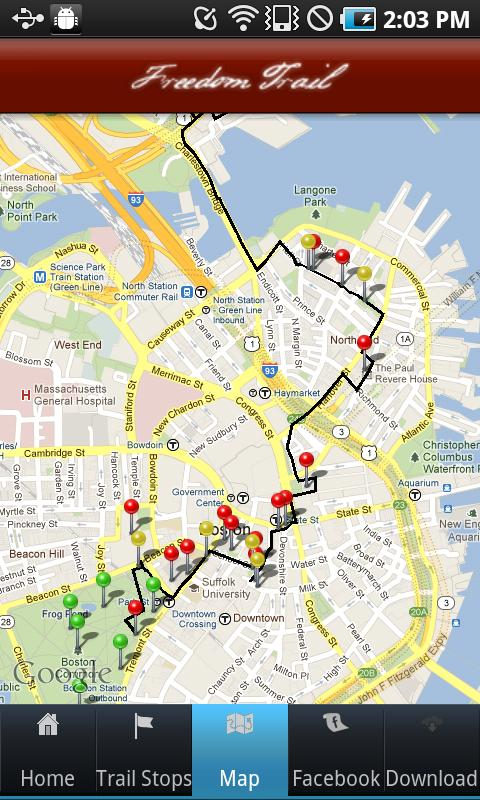
\includegraphics[width=1.0\linewidth]{./FreedomTrail}
\caption{The map screen of the Freedom Trail app. The app's user interface is well polished. However, it is tailor made for the highly specific Freedom Trail, and forces a user to download a very specific app for a very specific purpose, when a similar experience can be provided by a more inclusive app, thereby reducing the storage occupied by the app. }
\label{fig:FreedomTrail}
\end{figure}

We also looked at the mobile applications Geotour, YouVisit, TourBuddy, and MyTours. Like the applications mentioned above, these applications failed to successfully complement the tour taking experience; however, we did take note of a few features from each application that we enjoyed and wanted to implement in Campus Sherpa. We enjoyed: Geotour's location triggered changes, YouVisit's audio narration feature, TourBuddy's tour builder, and MyTours' tour browser. Figure~\ref{fig:GeoTour} illustrates the map feature of GeoTour that we really liked.

There also exists related academic work. A paper published by Zarmpou, Drosopoulou and Vlachopoulou titled \emph{Mapping the tourism mobile applications: what, how and where} \cite{Zarmpou:2013:MTM:2490257.2490295} examines fourteen mobile tourism applications and discusses their successes and downfalls, placing particular emphasis on the success and failures of their respective business models. 

\emph{Collective intelligence in toursplan: an online tourism social network with planning and recommendation services} published by Luz, Almeida, Anacleto, and Silva \cite{Luz:2013:CIT:2494444.2494449} examines the development of Toursplan, an information system backed by an online social network that provides tourists information about the areas they plan on touring. Toursplan analyzes social data to generate recommendations to their users as to which locations to visit and which tours to take. Although serving a different need of tourists, we took special note of how Toursplan took into account social data when making it's recommendations. 

\emph{Cyberguide: A mobile context-aware tour guide} published by Abowd, Atkeson, Hong, Long, Kooper, and Pinkerton \cite{Abowd:1997:CMC:272186.272199} discusses the development of Cyberguide, which, as the title of the paper suggests, was an early stab at providing tourists with a mobile, digital tour guide. Again, although Cyberguide aimed to solve a different tourism related problem than our application, we took note of their very well documented design and prototyping steps that led to their successful testing of Cyberguide.


\begin{figure}[h!]
\centering
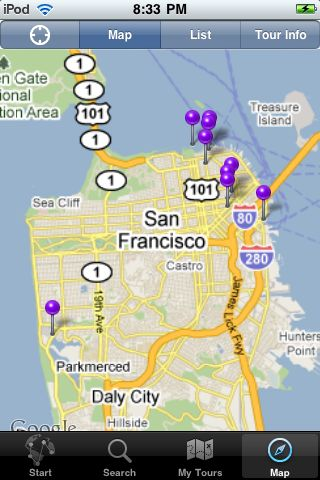
\includegraphics[width=1.0\linewidth]{./GeoTour}
\caption{The map screen of the GeoTour app. We chose to incorporate a similar element in Campus Sherpa}
\label{fig:GeoTour}
\end{figure}

\section{Background}

Motivated by the above observations, we first identified the types of people touring MIT. We decided that for the purposes of campus tours, we can broadly classify people as current students, prospective freshmen, parents, and tourists. In order to gather information about these groups, we conducted a survey of these four groups, with some questions common to all four groups and some tailored to a specific group. We reached out to tour groups, classmates/colleagues, and friends/family. Each participant was interviewed for approximately 15 to 20 minutes. Here are some of the questions we asked:

\textbf{Everyone}:

\begin{itemize}
	\item What is the most memorable site you've visited here? Why?
	\item What is the one thing you most wish to see here? Why?
	\item Have you gone on a tour of MIT?
	\begin{enumerate}
		\item Are there any questions the tour guide didn't answer?
		\item Did the tour take you everywhere you wanted?
		\item Did the tour leave out any place you wanted to see?
	\end{enumerate}
\end{itemize}

\textbf{Current Students}:
\begin{itemize}
	\item What are three things you looked for when touring MIT?
	\item What is one place that the tour didn't cover, which you think tourists should see?
\end{itemize}

\textbf{Prospective Freshman}:
\begin{itemize}
	\item If you could ask a current student one question about MIT, what would it be?
	\item What aspect of MIT do you want explore the most?
\end{itemize}

\textbf{Parents}:
\begin{itemize}
	\item What are three places you want to tour at MIT that you think your child might not want to?
	\item If you could ask a current student one question about MIT, what would it be?
\end{itemize}

\textbf{Tourists}:
\begin{itemize}
	\item How long will you be visiting MIT?
	\item In a sentence, why did you want to come visit MIT?
\end{itemize}

Approximately twenty people responded to the survey, evenly distributed across the four demographics. Some of the responses to the survey were:

``There are always too many things to see \ldots I am wishing I can see more later'' (current student)

``Campus Preview Weekend (CPW) was really rushed, and I did not get to see everything'' (prospective freshman)

``I wish I could get a better sense of MIT culture. The tour guide briefly touched on how each dorm was different, but did not go into detail. '' (prospective freshman)

``I wish they had shown us where the students hang out '' (parent)

``I wish I could get a better sense of MIT culture. The tour guide briefly touched on how each dorm is different, but didn't go into detail. '' (tourist)

From the above responses, we saw that a common complaint was that people were not able to visit places they wanted to with the regular campus tours. In order to solve this problem, we proposed an application that helps create and share custom tours of the MIT campus called ``Campus Sherpa''.

Since smartphones offer location awareness and mobility, they are the obvious platform choice for ``Campus Sherpa''. By deploying this application for iOS, users can take out their smartphone when they arrive at MIT, select a tour based on their interest, and then begin exploring sites that will be most useful to them.

The second aspect of ``Campus Sherpa'' that we wished to support is to allow users to chronicle their tours and share them with others. As prospective students compare MIT to other schools or as tourists reminisce about their visit to MIT, the ability to record their tours (by associating locations with text, photos, videos, and links to related content) will aid them in remembering. For current students, this offers a way to record the precious memories they make at MIT and share them with others. Thus, the primary audience will be people who aim to tour MIT and record their experience there. The secondary audience will be current MIT students who would like to chronicle their lives at MIT.

While some MIT tours will be pre-installed, the majority are intended to be user-created.
Based on our own experiences and the responses to our survey, people have varied tastes and desired destinations when visiting MIT, and we aimed to make sure that their trips to MIT are as enjoyable and productive as possible.

By creating an application to let users create, share, and follow custom tours of MIT, we hope to make college tours custom fit to each person's taste, to make memories of MIT easy to record and share, and to make a platform for sharing tours.

\section{System Description}

``Campus Sherpa'' allows users to achieve two goals: 

\begin{itemize}
	\item Take custom tours
	\item Create tours based on experiences.
\end{itemize}

When users launch the application, they are presented with a screen (Figure \ref{fig:TourBrowser}) that lists all tours that have been created (by any user). If they would like to take a tour, they can select one from the list, and they will be directed to a ``Start Tour'' page (Figure \ref{fig:TourPreview}), which includes a map of all of the locations on the tour. If any of the location pins are clicked, the name of the corresponding location is shown.

\begin{figure}
\centering
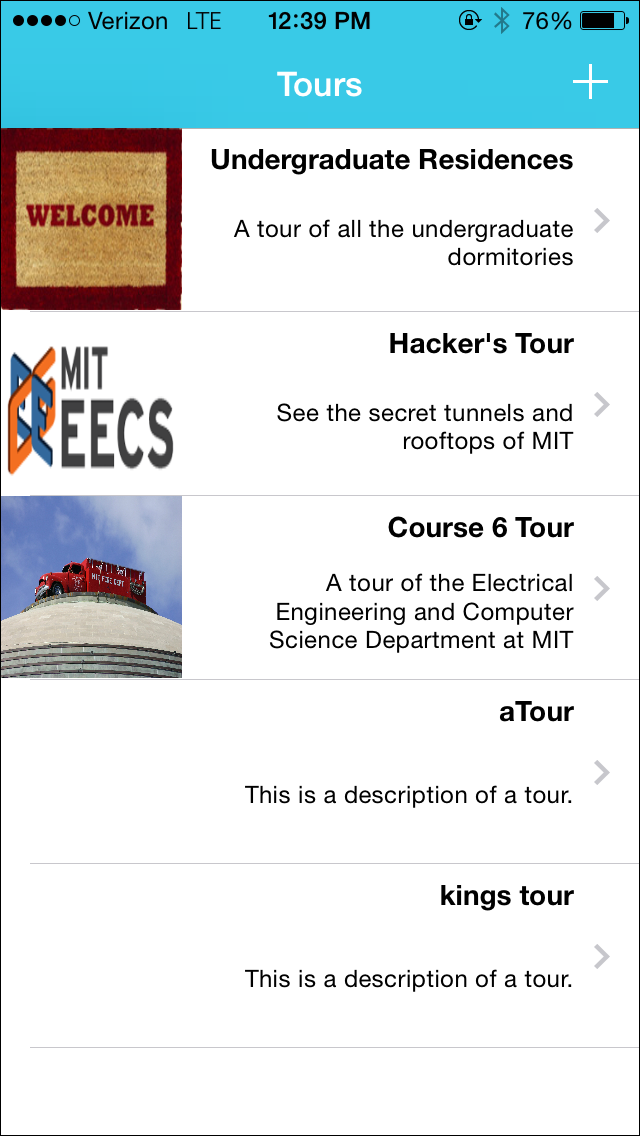
\includegraphics[width=0.7\linewidth]{./TourBrowser}
\caption{The tour browsing screen.}
\label{fig:TourBrowser}
\end{figure}


\begin{figure}
\centering
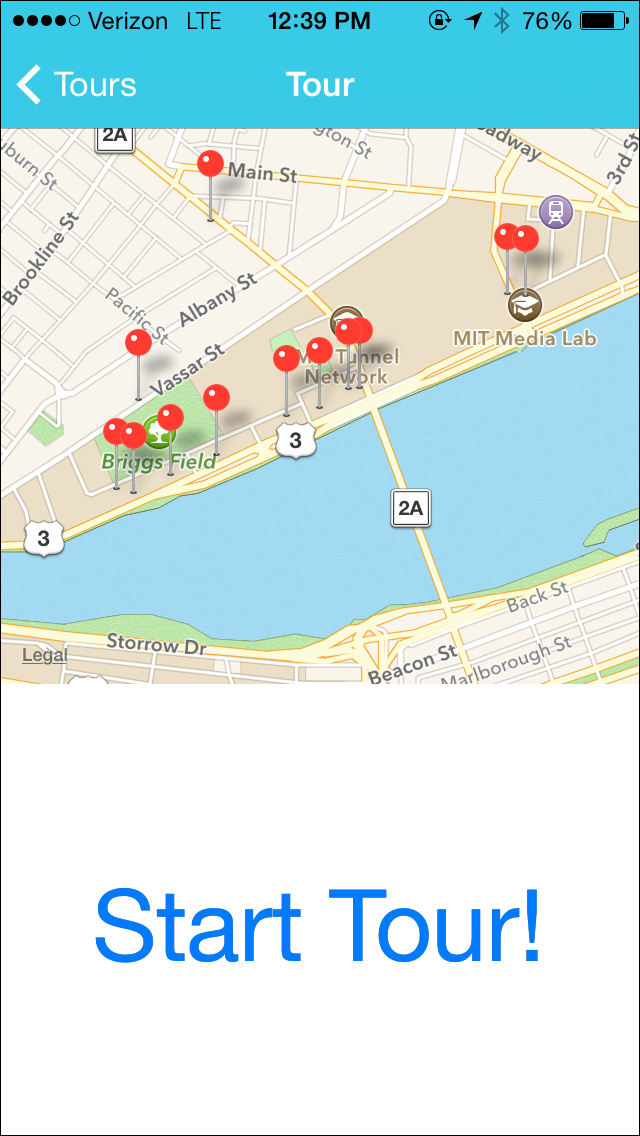
\includegraphics[width=0.7\linewidth]{./TourPreview}
\caption{The tour preview screen.}
\label{fig:TourPreview}
\end{figure}

Once the user starts a tour, they are presented with a screen for the first location. The screen contains a picture of the location, two buttons for navigating to the previous location and the next location, another button that brings up a map with all of the locations (the same map from Figure \ref{fig:TourPreview}), and a final button for the related media (Figure \ref{fig:LocationScreen}). The ``Show Map'' button has been included based on the field study - users indicated that they wanted to have access to the map of locations at all times.


\begin{figure}
\centering
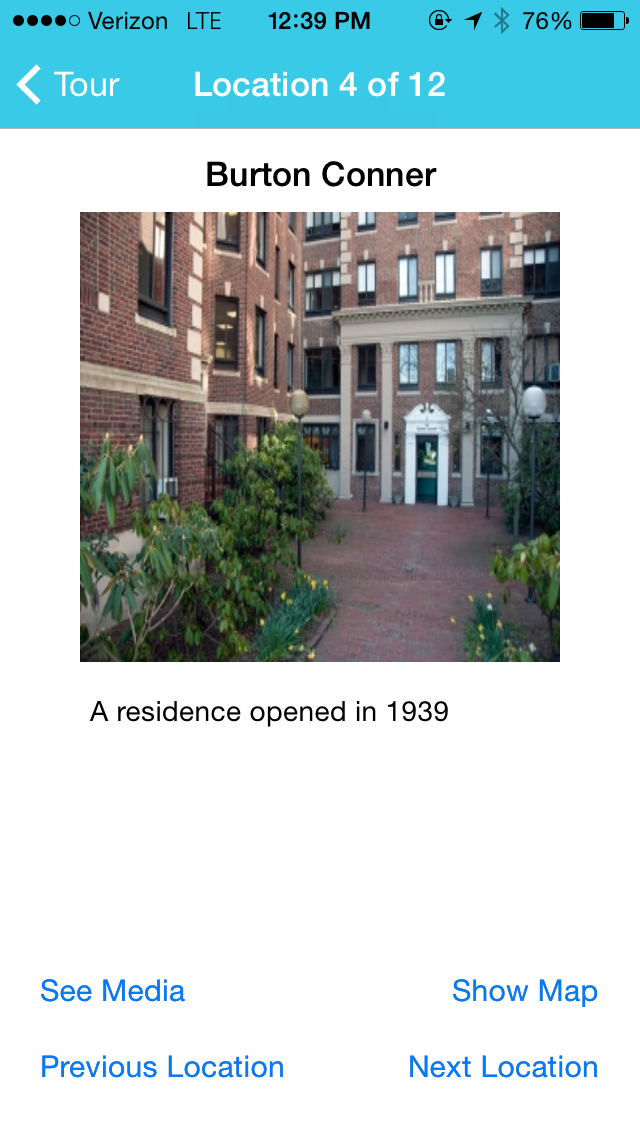
\includegraphics[width=0.7\linewidth]{./LocationScreen}
\caption{The location screen.}
\label{fig:LocationScreen}
\end{figure}

If the user clicks ``See Media'', then a list of media is displayed (Figure \ref{fig:MediaList}). The media includes images (such as pictures of the location) with descriptions. It also includes audio narration that can describe the locations. Based on user testing, we found that users wanted some form of audio in the tour. We experimented with text-to-speech and found that it sounded robotic and often mispronounced words. So, we decided to support audio narration instead, so that users can record descriptions of the location, which would be more natural than text-to-speech. The screen for listening to audio is displayed in Figure \ref{fig:AudioRecord} (the screen for recording audio is similar).

\begin{figure}
\centering
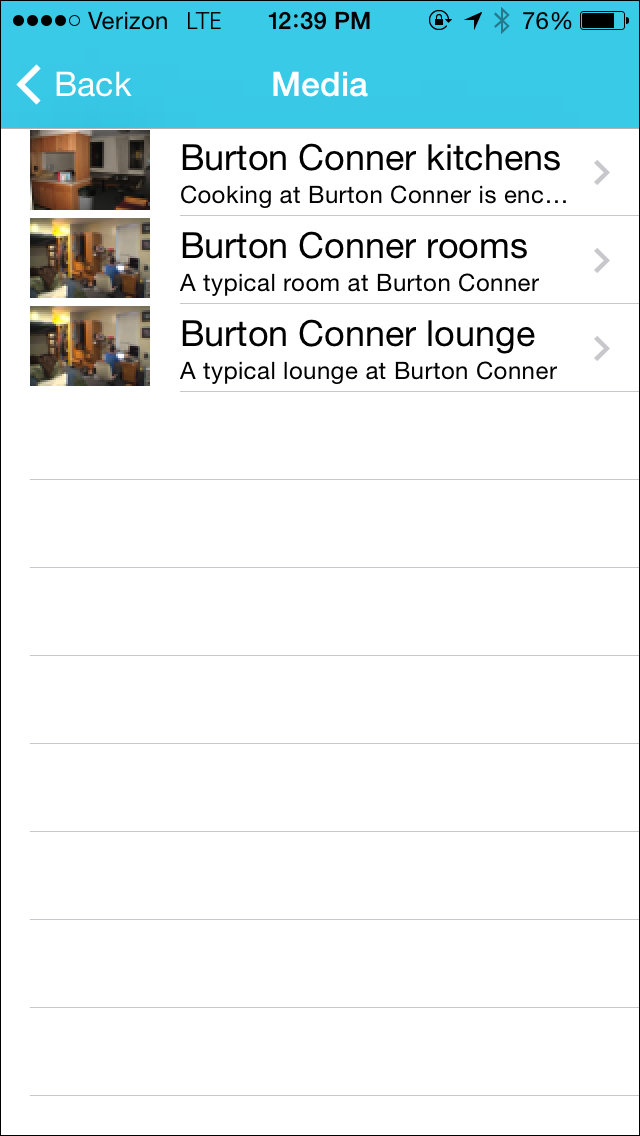
\includegraphics[width=0.7\linewidth]{./MediaList}
\caption{The media list for a given location. It can contain images and audio narration.}
\label{fig:MediaList}
\end{figure}

\begin{figure}
\centering
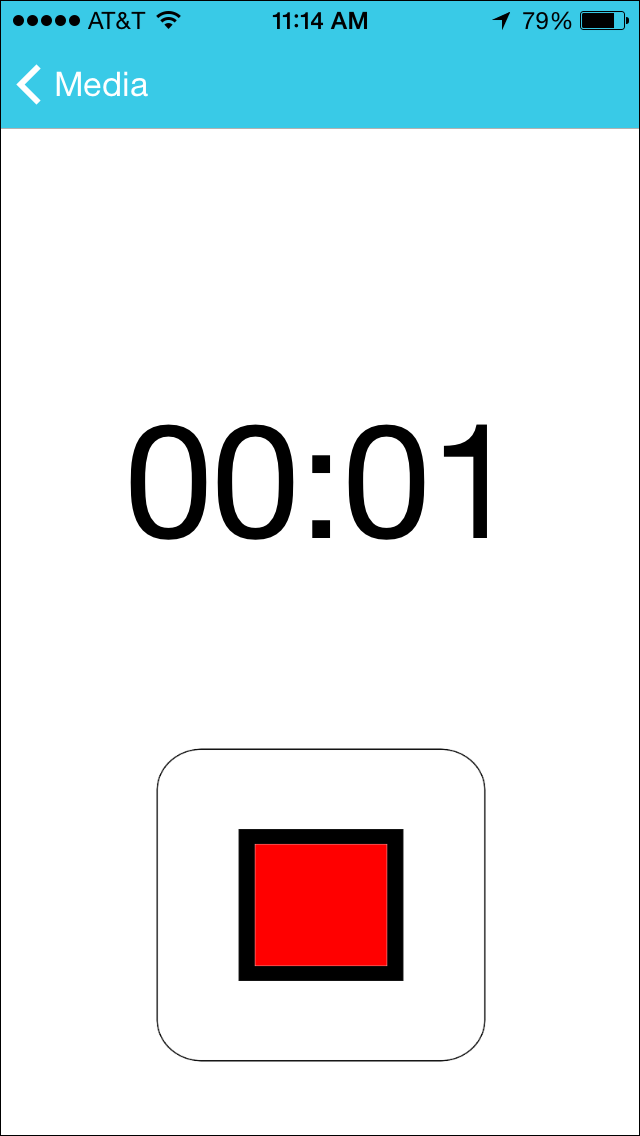
\includegraphics[width=0.7\linewidth]{./AudioRecord}
\caption{Users can record audio for tours.}
\label{fig:AudioRecord}
\end{figure}

The second part of Campus Sherpa is the tour creation aspect. Initially, tour creation was done in just two screens, but field testing showed that users were confused by the large number of UI elements on one screen. So, the app was updated and tour creation was broken into multiple screens. For instance, Figure \ref{fig:TourName} asks the user to enter the tour name.

\begin{figure}
\centering
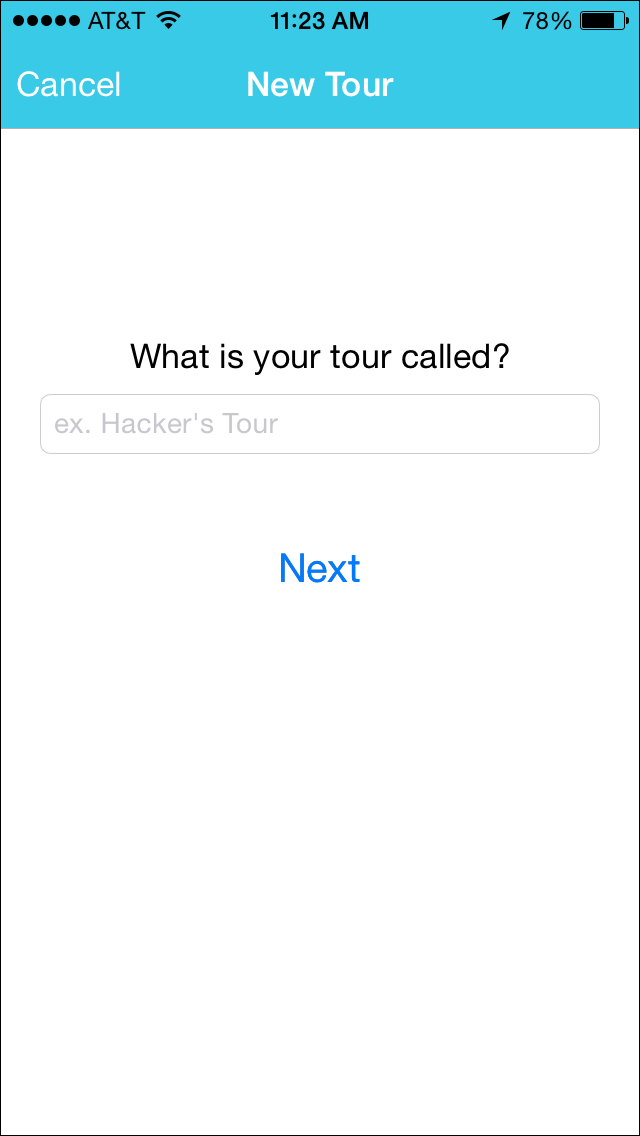
\includegraphics[width=0.7\linewidth]{./TourName}
\caption{Tour creation is broken into simple screens}
\label{fig:TourName}
\end{figure}

Then, the user enters the location. To simplify location entry, we either utilize the GPS to identify the user's current location (i.e. ``Use Current Location'') or we allow the user to enter the address (i.e. ``Use Above Address''). The address is converted to a latitude/longitude pair using the Google Maps API. The location entry screen is shown in  Figure \ref{fig:EnterLocation}. By modifying the tour creation mechanism as described, users were able to create tours with less difficulty and were more easily able to navigate through the app.

\begin{figure}
\centering
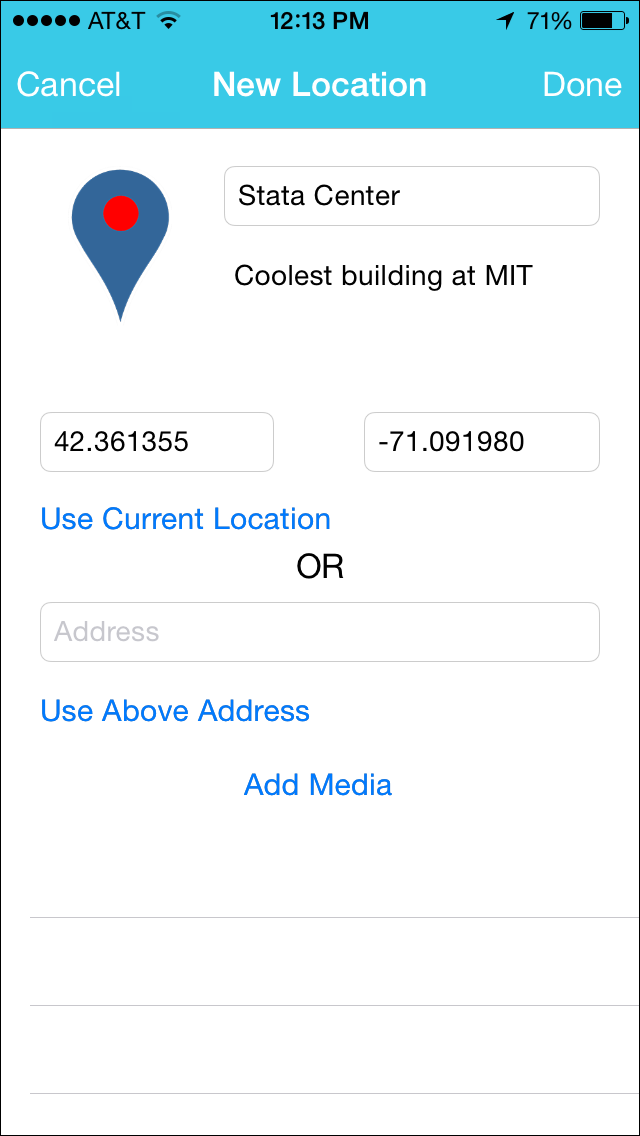
\includegraphics[width=0.7\linewidth]{./EnterLocation}
\caption{Location entry via address or GPS} 
\label{fig:EnterLocation}
\end{figure}

\subsection{Technical Details}
We use Parse for the backend. Parse is a backend-as-a-service which provides an SDK for iOS which allows users to persist objects in tables on the server. We chose Parse because it provided all the backend infrastructure we needed and it allowed us to focus on the interface and usability of the app. On Parse, we persist four kinds of objects:

\begin{itemize}
\item \textbf{Tour}, which consists of a name, description, thumbnail, and list of locations
\item \textbf{TourLocation}, which consists of a latitude/longitude pair, name, description, thumbnail, and list of media
\item \textbf{TourMedia}, which consists of a name, description, image, and audio. 
\item \textbf{Log}, which consists of a User ID, message, and time
\end{itemize}

We utilized Parse Analytics and Parse queries to analyze usage statistics and log messages. 

The application is implemented for iOS 7 using the Objective-C programming language. The application is designed using native UI controls (paper prototyping showed that users were not able to recognize custom controls). The layout and navigation were designed according to the Apple Human Interface Guidelines.
    
\section{Field Study}
Since our app is targeted at tourists of MIT, a demographic we did not have ready access to, we primarily focused on gathering information from two more readily available groups: iOS experts, who could critique the user experience of the app, and recent prefrosh (current MIT freshmen), who could assess the app's utility for prospective students. We had four students from each group take one tour (a brief tour of some locations in the Infinite Corridor) and make one tour, and we took notes on any difficulties they seemed to be experiencing while using the app. After they finished both tasks, we asked them for any feedback they had. We used a few standard questions:
\begin{itemize}
\item What additional features might it be useful for this app to have?
\item Was any part of the user experience awkward or difficult?
\item Do you see this app being useful in its current form to prospective tourists? What advantages would it have over tour guide-led tours?
\end{itemize}
We received a large volume of feedback. Some of the most common responses and insights follow:
\begin{itemize}
\item The ``Show Map'' screen (visible when taking a tour, looks much like Figure~ \ref{fig:TourPreview}) should have shown the pin for the current location in a different color.
\item The keyboard on many screens was hard to dismiss -- the iOS experts suggested converting many of the views to ScrollViews so that users could scroll down to see elements obscured by a keyboard.
\item If one location has a picture and the subsequent location does not (when taking a tour), the subsequent location's picture is set to the first location's picture, causing confusion.
\item The workflow for the make tour portion of the app was a bit confusing -- the ``Publish Tour'' button appeared too early, so users sometimes clicked it before adding any locations to the tour.
\item It would be nice if the app provided users directions to get one from one location to the next.
\end{itemize}
We modified the app to address the most common concerns of the testers. An interesting use case we discovered from running the field study is that many users actually like to step through tours in the app without actually moving physically from place to place. Thus, our app could prove incredibly useful to prospective students who are unable to visit the campus but want a sense for the rich variety of locations and sights at MIT. This use case could also help people plan what places they would like to visit during a trip to MIT. In essence, the app, if populated with a sufficient number of user-generated tours, could serve as a catalog of all of the interesting sets of related locations on campus.

After they tested the app, the testers were asked to fill out a brief survey consisting of the following questions, with responses being ratings on a 1-to-5 scale:
\begin{itemize}
\item How useful do you think this app would have been for you during CPW?, with 1 being ``Don't think tours would have played a big role in my decision, or tour guide-led tours would have been more than enough'' and 5 being ``Seeing different parts of campus would have been crucial to my decision, and this app would have helped me with that''
\item As a current MIT student, could you see yourself using this app to explore different parts of campus when you had some free time?, with 1 being ``Not at all'' and 5 being ``Definitely''
\item Could you see this app being useful to tourists who want to get a better sense of MIT?, with 1 being ``No, there are much better ways to do this'' and 5 being ``Yes, this app could offer much more information than tour guide-led tours or other options''
\end{itemize}
With the second question we explored yet another use case -- the physical tour for people who are already familiar with MIT in general but might want to explore a very niche part of campus. For example, there could be a tour with destinations popular for ``hacking'', which might include the roofs of various buildings and instructions on how to reach them. The results of this survey are plotted in Figure \ref{survey-results}. The results seem to indicate that users are very optimistic about the utility of the app to tourists, but are more skeptical about its usefulness to prospective undergraduates. This is reasonable, as it sounded from personal conversations that the CPW experience is more about meeting other future students than exploring every nook and cranny of the campus. The strong response to our second question also indicates that the use case for people already familiar with MIT is legitimate.

\begin{figure}
\centering
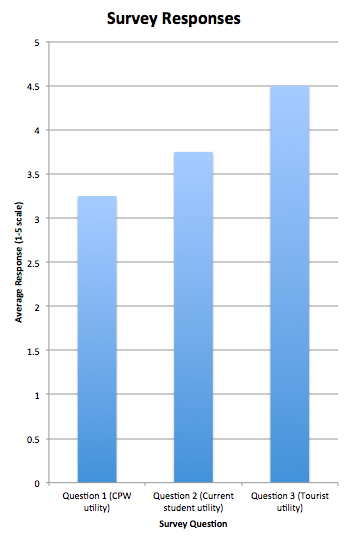
\includegraphics[width=1.0\linewidth]{./survey-responses.png}
\caption{Average responses, on 1-to-5 scale, to our survey questions.}
\label{survey-results}
\end{figure}

We also added quite a bit of logging to the code for our app. A summary of the logging output over all uses of the app by testers is shown in Tables~\ref{logging-results-take} and ~\ref{logging-results-make}. There are many interesting conclusions we can derive from this data. Starting with Table \ref{logging-results-take}, we can see that the ``See Media" button (``Opened media list") was clicked on at least one location in fewer than half of the cases where a tour was taken (``Started taking a tour"). This tells us that the ``See Media" button should have been made more prominent.

Looking next at Table \ref{logging-results-make}, in many cases where a user started making a tour, he or she did not add any locations to the tour (``Adding location to tour", ``Finished adding location to tour"). This further corroborates the suggestions of testers that we make the ``Add Locations" button more visible on the initial make tour screen and make it more difficult to click the ``Publish Tour" button without adding any locations. Furthermore, it seems that testers used their current GPS location to specify the latitude / longitude coordinates of a new location more often than they explicitly entered a street address. This indicates that they often physically walked to the locations they wanted to add to their tours, which seems reasonable considering tours are meant to cover only locations on the MIT campus. In addition, only a third or fewer of the created tours included any images (``Finished adding image to tour"). We intend for all locations, and certainly all tours, to contain at least one image, so it seems that we should make the add image / media forms more central to the tour creation experience. Finally, there were many cancellations of created locations, which suggests that editing the state of a partially created location was so difficult that users decided to cancel the location altogether and start from scratch.

\begin{table}
\begin{tabular}{|l|l|}\hline
\textbf{Log Message} & \textbf{Count} \\ \hline
 Started taking a tour & 267 \\ \hline
 Opened media list & 116 \\ \hline
 Clicked on media item & 157 \\ \hline
 Going to next location & 377 \\ \hline
 Going to previous location & 594 \\ \hline
\end{tabular}
\caption{Log message counts over all uses of the app for the take tour segment}
\label{logging-results-take}
\end{table}

\begin{table}
\begin{tabular}{|l|l|}\hline
\textbf{Log Message} & \textbf{Count} \\ \hline
 Started making a tour & 114 \\ \hline
 Adding location to tour & 77 \\ \hline
 Entered address for new location & 12 \\ \hline
 Used current GPS location for new location & 38 \\ \hline
 Opened add media view for new location & 69 \\ \hline
 Taking new picture to add to tour & 17 \\ \hline
 Choosing image from library to add to tour & 13 \\ \hline
 Cancelled library image picker & 5 \\ \hline
 Finished adding image to tour & 37 \\ \hline
 Cancelled out of add image view & 6 \\ \hline
 Finished adding location to tour & 42 \\ \hline
 Cancelled adding location to tour & 87 \\ \hline
 Cancelled create tour & 49 \\ \hline
\end{tabular}
\caption{Log message counts over all uses of the app for the make tour segment}
\label{logging-results-make}
\end{table}

\section{Discussion}

The next steps for Campus Sherpa are incredibly exciting. With the results form our field study in hand, we've developed a plan of action for further development of our application. We've also reflected on the process of developing Campus Sherpa and have outlined a few key takeaways from the experience, applicable not just to the development of a tourism related mobile application, but to more general application development as well.

Additionally, the findings of our research questions are of importance not just to us, but to the mobile tourism industry as well. Properly understanding which features in a mobile application work well with tourism is of paramount importance to successfully improving the tour taking experience by way of mobile technology.

Our findings are particularly relevant to the work published by Zarmpou, Drospoulou, and Valchopoulou  \cite{Zarmpou:2013:MTM:2490257.2490295}. In \emph{Mapping the tourism mobile applications: what, how and where}, they examined the successes and shortcoming of fourteen mobile tourism applications. Though this paper focused primarily on the business strategies behind each application, they did look into how each application was either successful or unsuccessful in improving upon the tour taking experience. From our field study, we were able to get a better understanding of how tourists interact with technology, something Zarmpou, Drospoulou, and Valchopoulou would likely find of interest, particularly our quantitative data. Additionally, our research and development of Campus Sherpa demonstrate just how far mobile technology has come in the last twenty years. Although our application was suited to enhance the tour taking experience by way of serving custom made tours instead of providing users with a virtual tour guide, Campus Sherpa extends on some of the work done for Cyberguide, a mobile context-aware tour guide developed by Abowd, Atkeson, Hong, Long, Kooper, and Pinkerton in 1997 \cite{Abowd:1997:CMC:272186.272199}.

\section{Future Work}

As can be seen from the field study, although a number of the key objectives of Campus Sherpa were met, a number of improvements are possible. 

From a technical standpoint, the user interface could be improved to make it look more professional. Although our UI has the advantage of being simplistic, with the addition of more features such as video, the UI might need to be reworked. For instance, to increase interface safety, a mechanism for managing tour creation (ex. save, undo, redo) could be implemented. Another technical improvement is the creation of our own backend for the app. For the purposes of the field study and initial deployment, we chose to use the Parse framework. Parse greatly accelerates the rate at which one can get an initial app deployed and running, and eliminates the need for managing the backend with its associated servers and databases ourselves. Moreover, Parse provides excellent data visualization and logging tools that greatly simplified the initial deployment of the app and the collection of data from the field study. However, as Campus Sherpa reaches more users, we believe it would be beneficial to switch to writing our own backend because of Parse's pricing and for the advantages of relying on our own infrastructure. Yet another advantage of using our own backend is that it makes the performance characteristics and bottlenecks of the app transparent to us. We did not receive any negative feedback regarding performance from our field study, but we do anticipate running into performance issues as the app reaches more users. 

A relatively simple change that should help in making Campus Sherpa reach more users and improve their experience with it is the addition of video to tour media, since at the moment Campus Sherpa supports only text and audio. Video is a key element in most of the related tourism apps that we examined in the related work section, and the results of our field study as well as feedback from others suggested that we should include it. Another related feature that could be of great benefit to the visually impaired is the addition of text to speech capabilities to the application. 

The next major milestone for Campus Sherpa is to create a recommendation system which suggests tours (or perhaps combine existing tours) that cater to a user's unique interests. This was omitted from this version of Campus Sherpa because 1) There weren't enough tours such that a recommendation system would be useful, and 2) The algorithmic and machine learning challenges of building a recommendation system were outside the scope of the class. Moreover, we felt that they were too complex for a proof of concept application. 

In similar spirit to the recommendation system is the integration of popular social applications such as Twitter and Facebook. This will enable users and tour creators to utilize the existing vast reach of networks such as Facebook to advertise a newly created tour. The success of Campus Sherpa is closely tied to the spread of awareness about it, because with very few users, not many tours get published and with a lack of good tours, one of the main purposes of Campus Sherpa is defeated. We believe that social networks can play a critical role in making a large number of people aware of the app and its capabilities. 

Another possible improvement suggested by our TA is making the user's location a more integral part of the app. Right now, the app can be run in ``armchair tourism'' mode, where a user simply sits somewhere and browses through all available tours. This is positive in some respects, since it allows users to view the available tours prior to experiencing them firsthand on campus. However, this comes at the cost of a loss in immersion. One way to address this is the creation of a new mode where users can take a tour ``realistically''. For instance, only tour locations near the user's current geographic location can be highlighted, and the rest are grayed out/disabled. 

\section{Conclusion}

The development of Campus Sherpa, all the way from prototyping and idea generation early in the term to software development and field testing a few weeks ago, was a truly eye opening experience. Over the term, we were able to develop a better understanding of how people interact with their mobile technology and how a well developed application can enhance the user's experience with not only that technology, but with the world around them as well. We are proud to have successfully developed a mobile application that enhances the tourist experience at MIT and are looking forward to further polishing our application, adding features, and going through further testing. More importantly, we look forward to gaining even more insight into human interaction with mobile technology through this further development. 



\section{Acknowledgments}

We would like to thank our TA Jason Martin Lipshin for guidance as well as constructive feedback. 

We would also like to thank the graduate students of Research Laboratory of Electronics and the Laboratory for Information And Decision Systems for their participation in the initial study. They gave us a unique perspective about campus tourism from the eyes of graduate students. We are also grateful to all the freshmen, parents, and tourists who also participated in the initial study. Interactions with the users of our study formed the basis of our key insight that there are multiple categories of people with different needs and expectations from a campus tourism application. Thus, they played a pivotal role in the shaping of our application. 

Additionally, we would like to thank the various participants in our field study. In particular, we wish to acknowledge the contributions of Arjun Srinivasan and Nick Locascio whose extensive knowledge of iOS application development helped us in our rapid iterations. 

Last but not least, we would like to thank Ed Barrett and Frank Bentley for providing us with the opportunity to pursue this project. They gave us great insight into how to develop an
application communicating with mobile technology and gave us the technical background to actually develop an iOS application with network and location services in use. 

% Balancing columns in a ref list is a bit of a pain because you
% either use a hack like flushend or balance, or manually insert
% a column break.  http://www.tex.ac.uk/cgi-bin/texfaq2html?label=balance
% multicols doesn't work because we're already in two-column mode,
% and flushend isn't awesome, so I choose balance.  See this
% for more info: http://cs.brown.edu/system/software/latex/doc/balance.pdf
%
% Note that in a perfect world balance wants to be in the first
% column of the last page.
%
% If balance doesn't work for you, you can remove that and
% hard-code a column break into the bbl file right before you
% submit:
%
% http://stackoverflow.com/questions/2149854/how-to-manually-equalize-columns-
% in-an-ieee-paper-if-using-bibtex
%
% Or, just remove \balance and give up on balancing the last page.
%
\balance

%\section{References}
%
%Theodora Zarmpou, Charoula Drosopoulou, and Maro Vlachopoulou. 2013. Mapping the tourism mobile applications: what, how and where. In Proceedings of the 6th Balkan Conference in Informatics (BCI '13). ACM, New York, NY, USA, 206-212. DOI=10.1145/2490257.2490295 http://doi.acm.org/10.1145/2490257.2490295
%
%Nuno Luz, Ana Almeida, Ricardo Anacleto, and Nuno Silva. 2013. Collective intelligence in toursplan: an online tourism social network with planning and recommendation services. InProceedings of the International C* Conference on Computer Science and Software Engineering(C3S2E '13). ACM, New York, NY, USA, 42-48. DOI=10.1145/2494444.2494449 http://doi.acm.org/10.1145/2494444.2494449
%
%Gregory D. Abowd, Christopher G. Atkeson, Jason Hong, Sue Long, Rob Kooper, and Mike Pinkerton. 1997. Cyberguide: a mobile context-aware tour guide. Wirel. Netw. 3, 5 (October 1997), 421-433. DOI=10.1023/A:1019194325861 http://dx.doi.org/10.1023/A:1019194325861

\bibliographystyle{acm-sigchi}
\bibliography{references}
\end{document}
